% Drawing 144/03-4 -- folder 144, batch 03, archive page 54 (PDF page 55).
% Transcription: Une figure à l'encre et au crayon : le complexe trivalent $K$ en traits gras (sommets marqués $0$), sa subdivision barycentrique en traits fins (sommets marqués $0$, $1$, $\infty$), et dix triangles-repères étiquetés $r$ (hachuré), $\tau_{0}r$, $\tau_{1}r$, $\tau_{\infty}r$, $\tau_{0}\tau_{1}r = \rho_{\infty}r$, $\tau_{1}\tau_{0}r = \rho_{\infty}r$, $\tau_{\infty}\tau_{1}r = \rho_{0}r$, $\tau_{0}\tau_{\infty}r = \rho_{0}^{-1}r$, $\tau_{0}\tau_{\infty}r = \tau_{\infty}\tau_{0}r = \rho_{1}r$, avec les sens de rotation et les flèches d'orientation des arêtes.
% Kind: trivalent complex K with barycentric subdivision and labelled frames. Method 2 (schematic redraw from the facsimile). Status: partial.
% Notes: Bold: the trivalent complex K (vertices 0). Thin: its barycentric subdivision (midpoints 1, face centres infinity). The ten frame labels are placed where they stand; their small rotation arrows and the arrowheads on the edges are not reproduced one by one. The struck strokes at the left and the left-hand legend ("le complexe topologique K ...") are not drawn.
% Coordinates: 1 unit = 1 mm = 1/100 of the crop width (bbox in page fractions: [0.2, 0.05, 0.62, 0.3]).
% Redrawn by Claude (claude-opus-5-5), issue #73, 2026-11-07; not checked by a human; not compiled (no TeX in the session).
% Rights: reproduces part of the work -- behind RENDER_TRANSCRIPTS, never published by itself.
\documentclass[tikz,border=3pt]{standalone}
\usepackage{amsmath,amssymb}
\usetikzlibrary{patterns,arrows.meta}
\tikzset{pencil/.style={black!45}, struck/.style={black!35}, mark/.style={circle,draw,inner sep=1.3pt}, pt/.style={circle,fill,inner sep=0.9pt}, opt/.style={circle,draw,fill=white,inner sep=1.1pt}}
\begin{document}
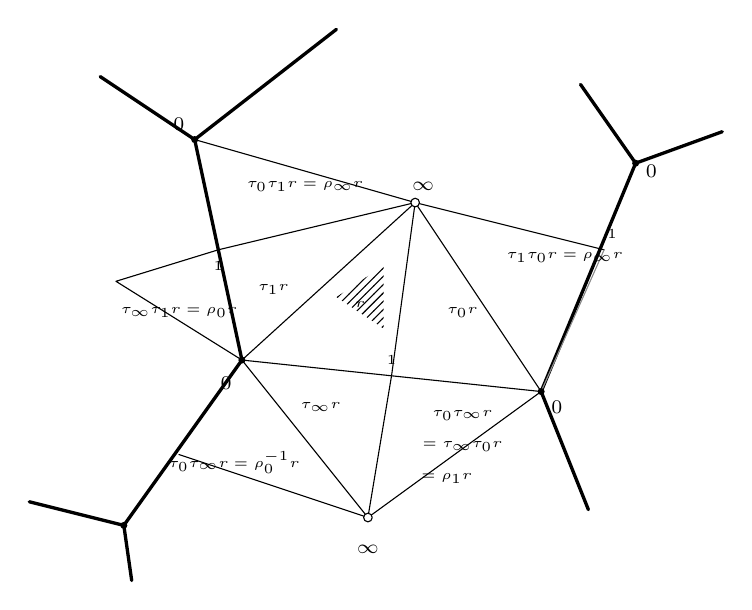
\begin{tikzpicture}[x=1mm,y=1mm,line cap=round,line join=round,font=\scriptsize]
\draw[very thick] (14,-16) -- (26,-24) -- (44,-10);
\draw[very thick] (26,-24) -- (32,-52);
\draw[very thick] (32,-52) -- (17,-73);
\draw[very thick] (5,-70) -- (17,-73) -- (18,-80);
\draw (32,-52) -- (70,-56);
\draw[very thick] (70,-56) -- (82,-27);
\draw[very thick] (75,-17) -- (82,-27) -- (93,-23);
\draw[very thick] (70,-56) -- (76,-71);
\draw (26,-24) -- (54,-32) -- (70,-56);
\draw (32,-52) -- (54,-32);
\draw (32,-52) -- (48,-72) -- (70,-56);
\draw (24,-64) -- (48,-72);
\draw (29,-38) -- (54,-32);
\draw (51,-54) -- (54,-32);
\draw (51,-54) -- (48,-72);
\draw (29,-38) -- (16,-42) -- (32,-52);
\draw (54,-32) -- (78,-38);
\draw[pencil] (78,-38) -- (70,-56);
\node[pt] at (26,-24) {};
\node[pt] at (32,-52) {};
\node[pt] at (70,-56) {};
\node[pt] at (82,-27) {};
\node[pt] at (17,-73) {};
\node[opt] at (54,-32) {};
\node[opt] at (48,-72) {};
\node[inner sep=1pt] at (24,-22) {\scriptsize $0$};
\node[inner sep=1pt] at (30,-55) {\scriptsize $0$};
\node[inner sep=1pt] at (72,-58) {\scriptsize $0$};
\node[inner sep=1pt] at (84,-28) {\scriptsize $0$};
\node[inner sep=1pt] at (55,-30) {\scriptsize $\infty$};
\node[inner sep=1pt] at (48,-76) {\scriptsize $\infty$};
\node[inner sep=1pt] at (29,-40) {\tiny $1$};
\node[inner sep=1pt] at (51,-52) {\tiny $1$};
\node[inner sep=1pt] at (79,-36) {\tiny $1$};
\node[inner sep=1pt] at (40,-30) {\tiny $\tau_0\tau_1 r=\rho_\infty r$};
\node[inner sep=1pt] at (36,-43) {\tiny $\tau_1 r$};
\node[inner sep=1pt] at (24,-46) {\tiny $\tau_\infty\tau_1 r=\rho_0 r$};
\node[inner sep=1pt] at (47,-45) {\tiny $r$};
\fill[pattern=north east lines] (44,-44) -- (50,-40) -- (50,-48) -- cycle;
\node[inner sep=1pt] at (60,-46) {\tiny $\tau_0 r$};
\node[inner sep=1pt] at (73,-39) {\tiny $\tau_1\tau_0 r=\rho_\infty r$};
\node[inner sep=1pt] at (42,-58) {\tiny $\tau_\infty r$};
\node[inner sep=1pt] at (31,-65) {\tiny $\tau_0\tau_\infty r=\rho_0^{-1}r$};
\node[inner sep=1pt] at (60,-59) {\tiny $\tau_0\tau_\infty r$};
\node[inner sep=1pt] at (60,-63) {\tiny $=\tau_\infty\tau_0 r$};
\node[inner sep=1pt] at (58,-67) {\tiny $=\rho_1 r$};
\end{tikzpicture}
\end{document}
